\documentclass[10pt]{article}

\usepackage{graphicx}
\usepackage[utf8]{inputenc}
\usepackage[spanish]{babel}
\usepackage{minted}
\usepackage{amsmath}
\usepackage[a4paper,top=2cm,bottom=2cm,left=3cm,right=3cm, marginparwidth=1.75cm]{geometry}
\usepackage{amsfonts}
\DeclareMathAlphabet{\pazocal}{OMS}{zplm}{m}{n}
\newcommand{\Lb}{\pazocal{L}}


\usemintedstyle{default}

\title{Práctica 1: Preeliminares, Gramáticas y
Expresiones Regulares}
\author{Miguel Ángel Dorado Maldonado}

\begin{document}
\maketitle

\section{Ejercicios}

\subsection{Calcula la potencia de la relación $R^3$ de $R = \{(1, 1), (1, 2), (2, 3), (3, 4)\}$.}

Partimos de
\[
R = \{(1, 1), (1, 2), (2, 3), (3, 4)\}.
\]

Primero calculamos $R^2 = R \circ R$:
\[
R^2 = \{(1, 1), (1, 2), (1, 3), (2, 4)\}.
\]

Ahora calculamos $R^3 = R^2 \circ R$. A partir de los pares de $R^2$:
\[
(1,1) \to (1,1), (1,2) \qquad
(1,2) \to (1,3) \qquad
(1,3) \to (1,4) \qquad
(2,4) \to 
\]

Por tanto,
\[
R^3 = \{(1, 1), (1, 2), (1, 3), (1, 4)\}.
\]

Resultado en python:

\begin{minted}{python3}
from libs.python.maths import power_relation

R = {(1, 1), (1, 2), (2, 3), (3, 4)}
R_cubed = power_relation(R, 3)
\end{minted}

\begin{center}
  \centering
  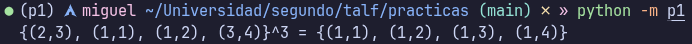
\includegraphics[width=0.8\textwidth]{assets/ej1.png}
\end{center}

\subsection{Dentro de la carpeta files, encuentra un fichero .tex cuyo contenido
incluya la cadena \textbackslash usepackage\{amsthm, amsmath\}}

Se usa el comando \texttt{grep} para buscar el fichero que contiene la cadena indicada
en todos los archivos indicando la expresión regular \texttt{files/*.tex}.

\begin{center}
  \centering
  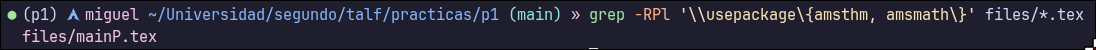
\includegraphics[width=0.8\textwidth]{assets/ej2.png}
\end{center}

El archivo que contiene la cadena es \texttt{files/mainP.tex}.

Demostración Proposición 1:
\begin{align*}
\Lb(((\alpha+\beta)\gamma))
  &= \Lb((\alpha+\beta))\Lb(\gamma) \\
  &= (\Lb(\alpha)\cup \Lb(\beta))\Lb(\gamma) \\
  &= \Lb(\alpha)\Lb(\gamma)\cup \Lb(\beta)\Lb(\gamma) \\
  &= \Lb((\alpha\gamma))\cup \Lb((\beta\gamma)) \\
  &= \Lb((\alpha\gamma+\beta\gamma)).
\end{align*}


Cadena que genera L:
\begin{center}
  \[
  \varepsilon + a + b + (a, b)^*(aa+ba+bb)
  \]
\end{center}

\newpage
\subsection{Modifica el fichero grammars.json del módulo grammar añadiendo una
nueva gramática y genera al menos 10 cadenas distintas de su lenguaje.}

La gramática elegida es la siguiente:

\begin{minted}{json}
{
  "name": "ejercicio3",
  "hint": "Gramática libre de contexto para expresiones aritméticas con suma, producto y paréntesis.",
  "e.g.": ["n", "n+n", "n*(n+n)"],
  "representation": {
    "N": ["E"],
    "T": ["n", "+", "*", "(", ")"],
    "P": [
      ["E", "n"],
      ["E", "(E+E)"],
      ["E", "(E*E)"]
    ],
    "S": "E"
  }
}
\end{minted}

Y el código Python utilizado para generar cadenas es:

\begin{minted}{python}
from python.grammar import produce

produce(
    "ejercicio3",
    num_strings=10,
    max_derivation=20,
    database_path="libs/python/grammar/grammars",
)

\end{minted}
Esto produce 10 cadenas del lenguaje generado aunque no se garantiza que
sean distintas ni terminales. Es por esto que se debe ejecutar varias veces
el código para que salgan distintas cadenas si terminales.
\newline

Cadenas generadas:
\begin{center}
  \centering
  \begin{tabular}{c|c}
    \texttt{n} & \texttt{(n+n)} \\
    \texttt{(n*n)} & \texttt{(n*(n+n))} \\
    \texttt{((n+n)*n)} & \texttt{((n*n)+n)} \\
    \texttt{((n+n)+n)} & \texttt{(n*(n*n))} \\
    \texttt{((n*n)*n)} & \texttt{((n+n)*(n+n))}
  \end{tabular}
\end{center}



\subsection{Diseña una expresión regular (en regexr.com o usando grep/Python) para
detectar direcciones de correo electrónico sencillas en un texto, e ilustra
su funcionamiento con ejemplos.}

He diseñado una expresión regular que detecta cualquier correo electrónico
con la forma 
\newline
\{combinacion mayus minus numeros\}@\{combinacion mayus minus
numeros\}.\{2 o mas caracteres\}.

\begin{center}
  \texttt{[A-Za-z0-9]+@+[A-Za-z0-0]+\textbackslash.[A-Za-z0-9]\{2,\}}
\end{center}

\begin{center}
  \centering
  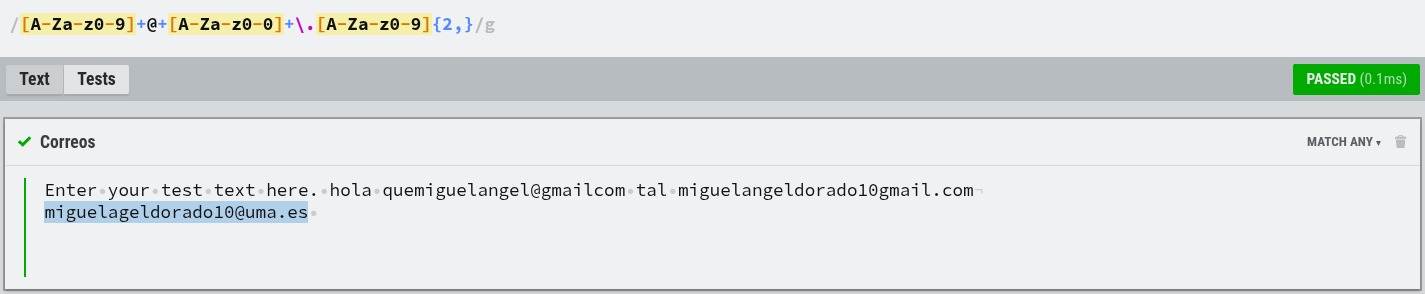
\includegraphics[width=1\textwidth]{assets/ej4.png}
\end{center}

\end{document}
